\documentclass[a4paper,10pt]{scrartcl}


\usepackage[utf8]{inputenc}


\usepackage{xcolor}
\definecolor{myblue}{cmyk}{1.00, 0.75, 0.00, 0.00}

\usepackage{tikz}
\usetikzlibrary{shapes,arrows,trees,decorations.pathmorphing,backgrounds,fit,shapes,arrows,chains, decorations.markings,shapes.arrows}
% \usepackage[a4paper]{geometry}

\renewcommand{\familydefault}{\sfdefault}
\usepackage[labelfont=bf]{caption}
\newcommand{\HRule}{\rule{\linewidth}{0.5mm}}
\setlength{\parindent}{0cm}

\def\MYTITLE{How I created a fully featured COMBINE archive}
\title{\MYTITLE}
\author{Martin Scharm}


\clubpenalty = 10000
\widowpenalty = 10000
\displaywidowpenalty = 10000

\usepackage{hyperref}
\hypersetup{
    bookmarks=true,
    unicode=false,
    pdftoolbar=true,
    pdfmenubar=true,
    pdffitwindow=false,
    pdfstartview={FitH},
    pdftitle={\MYTITLE},
    pdfauthor={martin scharm},
    pdfsubject={\MYTITLE},
    pdfcreator={martin scharm},
    pdfnewwindow=true,
    colorlinks=true,
    linkcolor=myblue,
    citecolor=myblue,
    filecolor=magenta,
    urlcolor=myblue
}

\bibliographystyle{alpha}

\begin{document}
\maketitle
% \thispagestyle{empty}
% \HRule \\[0.4cm]
% {\large Techreport, Tutorial, and Demo\\[.5em]}
% {\LARGE  \textbf{How I created a fully featured COMBINE archive}\\[.5em]}
% \HRule \\[1cm]
% 
% \begin{center}
% \Large
% Martin Scharm\\
% an probably others\\[8cm]\vfill
% \today\\
% \vfill
% \end{center}

\begin{abstract}
This is a small report on how I created the fully featured COMBINE archive
\href{https://github.com/SemsProject/CombineArchiveShowCase}{github.com/SemsProject/CombineArchiveShowCase}
to demonstrate the power of the COMBINE archive approach.
The developed COMBINE archive basically consists of (i) publication, (ii) model, (iii) simulation description, and (iv) simulation results.
The data encoded in the archive has shown that the developed simulation experiment is able to reproduce the results of a published study.
\end{abstract}



\section{Introduction}

The steadily increasing size and complexity of models and derived data poses the challenge of sharing reproducible results \cite{scharm2014}.
In times when collaborations over a distance of thousands of kilometres are mundane, researchers became aware of the importance of reproducibility \cite{Sandve2013}.
Therefore, there is an increasing demand for means to transfer simulation studies, ensuring reproducibility. CITE ro papers
Indeed, reproducibility is an essential challenge in systems biology \cite{Mesirov2010}.
In 2011 the pharmaceutical company Bayer tried to replicate published studies and failed in 64\% percent \cite{Prinz2011}.
Several projects and initiatives already deal with the problem of reproducibility, such as the Reproducibility Initiative\footnote{\href{http://reproducibilityinitiative.org/}{reproducibilityinitiative.org}} and FAIRDOM\footnote{\href{http://fair-dom.org/}{fair-dom.org}}.

Within the past decade the Computational Modeling in Biology Network (COMBINE) developed several standard formats to encode the different parts of a simulation study, such as SBML \cite{Hucka2003} and CellML \cite{Cuellar2003a} to encoded biological systems, SBGN \cite{sbgn} to encode visualisations, SED-ML \cite{Waltemath2011} to encoded the simulation setups, NuML\footnote{\href{https://github.com/numl/numl}{github.com/numl/numl}} and SBRML \cite{Dada2010} to encode numerical data and simulation results.
These markup languages allow for an encoding single parts of a model in an exchangeable format.
However, a simulation study usually consists of multiple files, the very model might be decomposed into various modules.
Transferring research results, thus, remained a challenge.

To close this gap, the COMBINE community developed the COMBINE archive, a single file that aggregates all the information necessary for a modelling and simulation experiment in biology \cite{Bergmann2014}.
The basis of the COMBINE archive is the Open Modeling EXchange format (OMEX), which bundles all the files that belong to an experiment.
Enriched with meta data, simulation experiments can reproducibly encoded in COMBINE archives.

To demonstrate the capabilities of a COMBINE archive I created a demo archive, which is available from our GitHub project\footnote{\href{https://github.com/SemsProject/CombineArchiveShowCase}{github.com/SemsProject/CombineArchiveShowCase}}.
In the following I describe what I did to build that archive.



\section{Methods}

The development of the fully featured COMBINE archive can be divided into three major parts.
I first decided for a simulation study to encode in an archive, then I created an initial archive which was then enriched with information I found on the internet and data that I generated on my own.
These steps are described in the following.

\subsection{Deciding for a Simulation Study}

I developed 3 criteria to decide for a simulation study:

\paragraph{Criteria 1: Open Access.}
As I want to share the demo archive openly, I had to decide for an experiment that offers as much open data as possible.
Obviously and unfortunately, the publication, as an essential document for the documentation of experiments, is the bottleneck.
Therefore, I needed to find a simulation experiment which was published using an open access license.

\paragraph{Criteria 2: Much data already available in standard formats.}
As I did not want to encoded the model myself, I restricted my search to studies which are already available as SBML and CellML models.
Ideally, these models are already curated, which increases my trust in the encoding.

\paragraph{Criteria 3: I have ideally already dealt with that publication.}
As I will need to work with the study I need to understand it.
It usually takes a lot of time to dig into a new field, so I preferred studies that I already investigated.
However, this was just a soft criteria to decrease my workload.


\paragraph{Searching for a matching study.}
Searching for a study was harder than I thought.
I failed to encoded my search criteria for the search engines of current databases.
I ended up asking a common search engine to look for names of open access journals at the websites of the databases and eventually \texttt{site:models.cellml.org "Molecular Systems Biology"}\footnote{\href{https://duckduckgo.com/?q=site\%3Amodels.cellml.org+\%22Molecular+Systems+Biology\%22}{duckduckgo.com/?q=site\%3Amodels.cellml.org+\%22Molecular+Systems+Biology\%22}} resulted in a model that is available from the CellML model repository (Calzone, Thieffry, Tyson, Novak, 2007\footnote{\href{http://models.cellml.org/exposure/1a3f36d015121d5596565fe7d9afb332}{models.cellml.org/exposure/1a3f36d015121d5596565fe7d9afb332}}) \cite{cellmlrepo} and from the Biomodels Database (BIOMD0000000144\footnote{\href{http://www.ebi.ac.uk/biomodels-main/BIOMD0000000144}{www.ebi.ac.uk/biomodels-main/BIOMD0000000144}}) \cite{biomodels}.


\paragraph{The final study.}
The study I chose was published by Calzone \emph{et.~al.} in Molecular Systems Biology. They propose a dynamical model for the molecular events underlying rapid, synchronous, syncytial nuclear division cycles in \textit{Drosophila} embryos \cite{Calzone2007}.
In an earlier study dealing with the cell cycle I already touched that publication, so it was the perfect study for the demo archive project.




\subsection{Creating an initial COMBINE archive}

\begin{figure}
\begin{center}
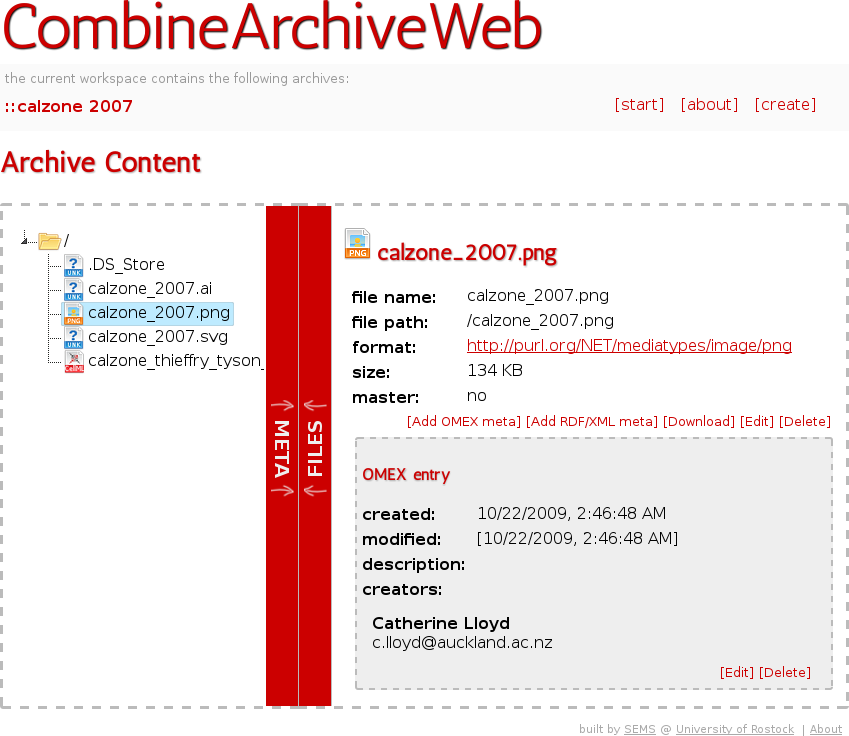
\includegraphics[width=.8\textwidth]{img/webcat-screenshot-combined.png}
\end{center}
\caption{The CombineArchiveWeb application showing the archive as it was exported from M2CAT. The files were cloned from the CellML model repository and immediately annotated with meta data. Thus, it is clear that I am not the creator of \textit{calzone\_2007.png}, instead it lists Catherine Lloyd as the creators and .}
\label{fig:screen:webcat}
\end{figure}

I created an initial version of the COMBINE archive using M2CAT \cite{m2cat}.
The webinterface as \href{http://m2cat.sems.uni-rostock.de/}{m2cat.sems.uni-rostock.de} searches in a graph database to retrieve links to models published in open databases \cite{masymos}.
The search for \texttt{Calzone} resulted in two matches, one of them representing the model in the CellML model repository.
In addition to searching in a graph database, M2CAT is also able to retrieve the files that correspond to a simulation study from other sources, such as open model repositories, and to bundle them in combine archives using the library of the CombineArchive Toolkit \cite{cat}.
The web interface also provides means to immediately explore the generated archive in the CombineArchiveWeb application \cite{scharm2014}.

In case of the Calzone \emph{et.~al.} study, the files of the CellML model repository were cloned and aggregated in a new COMBINE archive.
Additionally, the resulting archive and its files were annotated with all the meta data available from the GIT project of the CellML model repositories.
Specifically, the archive was annotated with the information that it was generated by M2CAT, and the files that were cloned from the CellML model repository are annotated with creators/contributors and modification times as available from the corresponding GIT project (\texttt{git log}), see Figure~\ref{fig:screen:webcat}. Thus, the an initial version of the COMBINE archive was obtained automatically and very quickly.






\subsection{Extending the COMBINE archive}
As the initial version only contains the model encoded in CellML together with some figures (all files exclusively from the CellML model repository) I needed to extend the archive manually.
To organize the files I developed a structure containing the following directories:
\begin{itemize}
 \item \texttt{model/}: files that encode an visualise the biological system
 \item \texttt{experiment/}: files that encode the \textit{in silico} setup of the experiment
 \item \texttt{documentation/}: files that describe and document the model and/or experiment
 \item \texttt{result/}: files that result from running the experiment
\end{itemize}

Using the CombineArchiveWeb application it was very easy to get rid of the unrelated \texttt{.DS\_Store} file. In the web interface I also moved all other files into the model directory, as they all encoded the mode.
The other directories are to be filled in the next sections.

\subsubsection{Retrieving Data and Information from other Services}
The first chapter of extending the archive dealt with a search for resources related to this study on the internet.

\paragraph{The article} is usually the central object of a research study. As I said earlier, Calzone \emph{et.~al.} published their findings in Molecular Systems Biology. So I went to the corresponding website\footnote{\href{http://msb.embopress.org/content/3/1/131}{msb.embopress.org/content/3/1/131}} and downloaded the article and supplementary information.
As both describe the experiment, I uploaded the files to the documentation directory in the CombineArchiveWeb application.
The web interface decently added meta data listing me as the creator of the file, which, unfortunately, is in this case incorrect.
Thus, I modified the entries to attribute the real creators and to state when and where the files where downloaded.
Additionally, I added modification dates to the meta data of these files by copying them from the website of the article and the meta data of the PDF files.
The CombineArchiveWeb application provides a nice interface to modify the meta data without knowledge about XML or RDF.
However, in the background it of course created a RDF/XML tree to describe the main article in a machine readable format, see section~\ref{sec:rdfmeta}.
This XML subtree was then added to the meta data file of the archive.


\paragraph{The model} encoded in SBML format was already available from the Biomodels Database, so I went there to retrieve the file \texttt{BIOMD0000000144.xml}\footnote{\href{http://www.ebi.ac.uk/biomodels-main/download?mid=BIOMD0000000144}{www.ebi.ac.uk/biomodels-main/download?mid=BIOMD0000000144}} (SBML level 2 version 1).
The model file was then also uploaded to the \texttt{model/} in the CombineArchiveWeb application and the meta data was modified to attribute the correct authors, curators, and contributors, according to the Biomodels Database website\footnote{\href{http://www.ebi.ac.uk/biomodels-main/BIOMD0000000144}{www.ebi.ac.uk/biomodels-main/BIOMD0000000144}} and as stated in the model document.


\subsubsection{Generating more Data}
The model files and the journal article are obviously not sufficient to reproduce the experiment's results, but I did not find any other information on the internet.
Thus, I generated more data myself.

\paragraph{The simulation description} is essential to run the experiment.
It defines the environment and the output of the \textit{in silico} execution.
Creating an initial simulation description was easy using the SED-ML Web Tools\footnote{\href{http://bqfbergmann.dyndns.org/SED-ML_Web_Tools}{bqfbergmann.dyndns.org/SED-ML\_Web\_Tools}} (SWT).
I just needed to upload the model and a ticking some boxes and the SWT created an initial SED-ML script which runs a time course simulation on the model and produces a graph for the concentration of every and the value of every parameter.


creating simulation description

\paragraph{The simulation results}
simulating it
storing results

\paragraph{The visualisation} of the model can be encoded in a standard format
generating sbgn compliant figure





\section{Results}

\subsection{The COMBINE archive}
During my work I kept the COMBINE archive in a GIT repository for version control.
The latest version of the archive can be found at GitHub\footnote{\href{https://github.com/SemsProject/CombineArchiveShowCase}{github.com/SemsProject/CombineArchiveShowCase}}.
At the time of writing this report\footnote{latest git commit: 2e946ce1adfd05d16350c30176e29546301603a2 -- 2015-06-11}, the archive consists of 25 files organizes in four directories (cmp. Section~\ref{sec:extendingarchive}), including the \texttt{manifest.xml} and \texttt{metadata.rdf} (the skeleton of the archive, see Section~\ref{sec:intro}) and a \texttt{README.md} file for the GitHub repository.
The manifest listing all ingredients of the COMBINE archive is attached in Section~\ref{sec:manifest}.

The archive basically consists of 4 modules: (i) the publication stored in the \texttt{documentation/} directory, (ii) the model of the biological system encoded in standardised formats stored in the \texttt{model/} directory, (iii) the simulation description encoded in SED-ML defining the simulation setup stored in the \texttt{experiment/} directory, (iv) the simulation results in form of graphs stored in the \texttt{result/} directory.
The files in these directories were either retrieved from other websites (publication, SBML model, CellML model) or generated especially for this archive (SED-ML scripts, simulation results, SBGN map).
The goal of this archive is to encode a reproducible simulation study.
Figure~\ref{fig:sim:results} has shown that the study developed is able to reproduce graphs 



\subsection{The Effort}







\section{Discussion}
The typical complexity of research results bears the challenge of transferring them in a way, that others are able to reproduce it.
Sharing your research results therefore involves a few problems.
% First, you need to identify and ship all relevant files.
% Only if your collaborators/readers have access to all the files 
Firstly, all relevant files need to be shipped.
Simulation studies usually consist of multiple relevant files, which are all necessary to run the experiment.
To reproduce a study it is essential to have access to all these files.
Secondly, users need to know the type and meaning of these files.
The files should be in standardized formats, so that the user has a chance (i) to grasp what is encoded inside, (ii) to understand how to use them, and (iii) to execute them in a software tool of their choice.
Especially, if the tool used to create the files is not available (anymore).
Thirdly, there must be a manual on how to use the files.
For example, the model might rely on modules and the simulation description might expect this model in at a certain location.
Thus, if the files are not arranged properly, the study cannot be rerun.
Fourthly, it must be clear who to consult in case of problems.
Users need to know who is/was responsible for a certain part of the simulation study.
Creators and contributors should be attributed appropriately.
As these requirements are crucial yet error-prone the COMBINE archive approach gives researches a hand.

A COMBINE archive is basically a container which is able to aggregate all files that are relevant for a simulation study.
The archive maintains a manifest listing its contents (files and their formats) and a some meta data describing the files and the archive itself.
Tools supporting COMBINE archives are able to understand its ingredients and can, for example, run the encoded experiment just as its creator intended run it.
Thus, users do not need to understand each of these files in detail.
They do not even need to know that the model is decomposed, or that it is encoded in, e.g., the SBML format.
Users just need the archive which provides all necessary information to rerun the experiment.

However, tool support for COMBINE archives is still very limited.
The experiment encoded in the developed archive is able to reproduce the figure published in the corresponding publication, see Figure~\ref{fig:sim:results}.
However, there is currently no tool able to consume the developed archive and run the experiment.
That's reasonable, as the standard of COMBINE archives is still very young.
We are in touch with different tool developers to fix problems and to increase tool support for COMBINE archives.
I hope that the archive developed in this study helps tool developers to implement support for COMBINE archives.


In the future I expect to see more tools able to read and export COMBINE archives.
It would support researchers in sharing and distributing their hard-earned scientific results.


% 
% As this approach is obviously very beneficial people are already convinced of it.
% 
% 
% 
% machts auch einfach. ein researcher muss nicht alle files verstehen, oder ueberhaupt wissen dass da ein model in eg. sbml encoded is. er braucht nur das archive, welches den simulationstools alle notwendigen infos liefert
% 
% 
% why is that useful?
% what's the advantage?
% space for improvements?
% 
% 
% outlook?



\section{Acknowledgements}




\bibliography{meta/refs}

  \setcounter{section}{0}%
  \renewcommand*\thesection{\Alph{section}}%
\section{Appendix}
\label{sec:appendix}

\subsection{The Mainfest}
\label{sec:manifest}
\begin{mdframed}[style=mddefault,frametitle={The \texttt{manifest.xml} of the final COMBINE archive}]
\begin{minted}[linenos,breaklines=true,numbersep=5pt,tabsize=2,xleftmargin=-7pt,fontsize=\footnotesize]{xml}
<?xml version="1.0" encoding="UTF-8"?>
<omexManifest xmlns="http://identifiers.org/combine.specifications/omex-manifest">
  <content location="." format="http://identifiers.org/combine.specifications/omex" />
  <content location="./manifest.xml" format="http://identifiers.org/combine.specifications/omex-manifest" />
  <content location="./README.md" format="http://purl.org/NET/mediatypes/text/x-markdown"/>
  <content location="./model/BIOMD0000000144.xml" format="http://identifiers.org/combine.specifications/sbml.level-2.version-1" />
  <content location="./model/calzone_2007.ai" format="http://purl.org/NET/mediatypes/application/illustrator" />
  <content location="./model/calzone_2007.png" format="http://purl.org/NET/mediatypes/image/png" />
  <content location="./model/calzone_2007.svg" format="http://purl.org/NET/mediatypes/image/svg+xml" />
  <content location="./model/calzone_thieffry_tyson_novak_2007.cellml" format="http://identifiers.org/combine.specifications/cellml" />
  <content location="./model/sbgn/Calzone2007.gml" format="http://purl.org/NET/mediatypes/text/plain" />
  <content location="./model/sbgn/Calzone2007.graphml" format="http://purl.org/NET/mediatypes/application/xml" />
  <content location="./model/sbgn/Calzone2007.png" format="http://purl.org/NET/mediatypes/image/png" />
  <content location="./model/sbgn/Calzone2007.pdf" format="http://purl.org/NET/mediatypes/application/pdf" />
  <content location="./experiment/Calzone2007-simulation-all-figures.xml" format="http://identifiers.org/combine.specifications/sed-ml.level-1.version-1" />
  <content location="./experiment/Calzone2007-simulation-figure-1B.xml" format="http://identifiers.org/combine.specifications/sed-ml.level-1.version-1" master="false"/>
  <content location="./documentation/Calzone2007.pdf" format="http://purl.org/NET/mediatypes/application/pdf" />
  <content location="./documentation/Calzone2007-supplementary-material.pdf" format="http://purl.org/NET/mediatypes/application/pdf" />
  <content location="./result/Fig1B-top-webtools.png" format="http://purl.org/NET/mediatypes/image/png" />
  <content location="./result/Fig1B-bottom-webtools.png" format="http://purl.org/NET/mediatypes/image/png" />
  <content location="./result/Fig1B-top-COPASI.svg" format="http://purl.org/NET/mediatypes/image/svg+xml" />
  <content location="./result/Fig1B-bottom-COPASI.svg" format="http://purl.org/NET/mediatypes/image/svg+xml" />
  <content location="./metadata.rdf" format="http://identifiers.org/combine.specifications/omex-metadata" />
</omexManifest>
\end{minted}
\end{mdframed}


\subsection{RDF/XML meta data snippets}
\label{sec:rdfmeta}
\begin{mdframed}[style=mddefault,frametitle={Meta Data of the Publication \texttt{Calzone2007.pdf}}]
\begin{minted}[linenos,breaklines=true,numbersep=5pt,tabsize=2,xleftmargin=-7pt,fontsize=\footnotesize]{xml}
<rdf:Description rdf:about="/documentation/Calzone2007.pdf">
	<dcterms:description>Article published in Mol Syst Biol. 2007; 3: 131. DOI:  10.1038/msb4100171, downloaded June 11th, 2015 . It describes the models /model/calzone_thieffry_tyson_novak_2007.cellml and /model/BIOMD0000000144.xml .</dcterms:description>
	<dcterms:creator>
		<rdf:Bag>
			<rdf:li rdf:parseType="Resource">
				<vCard:n rdf:parseType="Resource">
					<vCard:family-name>Calzone</vCard:family-name>
					<vCard:given-name>Laurence</vCard:given-name>
				</vCard:n>
				<vCard:org rdf:parseType="Resource">
					<vCard:organization-name>Molecular Network Dynamics Research Group of Hungarian Academy of Sciences and Budapest University of Technology and Economics, Budapest</vCard:organization-name>
				</vCard:org>
			</rdf:li>
		</rdf:Bag>
	</dcterms:creator>
	<dcterms:creator>
		<rdf:Bag>
			<rdf:li rdf:parseType="Resource">
				<vCard:n rdf:parseType="Resource">
					<vCard:family-name>Thieffry</vCard:family-name>
					<vCard:given-name>Denis</vCard:given-name>
				</vCard:n>
				<vCard:org rdf:parseType="Resource">
					<vCard:organization-name>Université de la Méditerranée, Campus Scientifique de Luminy, Case 928, Marseille, France</vCard:organization-name>
				</vCard:org>
			</rdf:li>
		</rdf:Bag>
	</dcterms:creator>
	<dcterms:creator>
		<rdf:Bag>
			<rdf:li rdf:parseType="Resource">
				<vCard:n rdf:parseType="Resource">
					<vCard:family-name>Tyson</vCard:family-name>
					<vCard:given-name>John J</vCard:given-name>
				</vCard:n>
				<vCard:org rdf:parseType="Resource">
					<vCard:organization-name>Department of Biological Sciences, Virginia Polytechnic Institute and State University, Blacksburg, VA, USA</vCard:organization-name>
				</vCard:org>
			</rdf:li>
		</rdf:Bag>
	</dcterms:creator>
	<dcterms:creator>
		<rdf:Bag>
			<rdf:li rdf:parseType="Resource">
				<vCard:n rdf:parseType="Resource">
					<vCard:family-name>Novak</vCard:family-name>
					<vCard:given-name>Bela</vCard:given-name>
				</vCard:n>
				<vCard:email>bela.novak@bioch.ox.ac.uk</vCard:email>
				<vCard:org rdf:parseType="Resource">
					<vCard:organization-name>Molecular Network Dynamics Research Group of Hungarian Academy of Sciences and Budapest University of Technology and Economics, Budapest</vCard:organization-name>
				</vCard:org>
			</rdf:li>
		</rdf:Bag>
	</dcterms:creator>
	<dcterms:created rdf:parseType="Resource">
		<dcterms:W3CDTF>2007-01-08T00:00:00Z</dcterms:W3CDTF>
	</dcterms:created>
	<dcterms:modified rdf:parseType="Resource">
		<dcterms:W3CDTF>2007-01-08T00:00:00Z</dcterms:W3CDTF>
	</dcterms:modified>
	<dcterms:modified rdf:parseType="Resource">
		<dcterms:W3CDTF>2007-06-22T00:00:00Z</dcterms:W3CDTF>
	</dcterms:modified>
	<dcterms:modified rdf:parseType="Resource">
		<dcterms:W3CDTF>2007-07-24T08:58:57Z</dcterms:W3CDTF>
	</dcterms:modified>
	<dcterms:modified rdf:parseType="Resource">
		<dcterms:W3CDTF>2014-03-26T11:22:15Z</dcterms:W3CDTF>
	</dcterms:modified>
</rdf:Description>
\end{minted}
\end{mdframed}

\end{document}
